\begin{figure} [H]
	\centering
	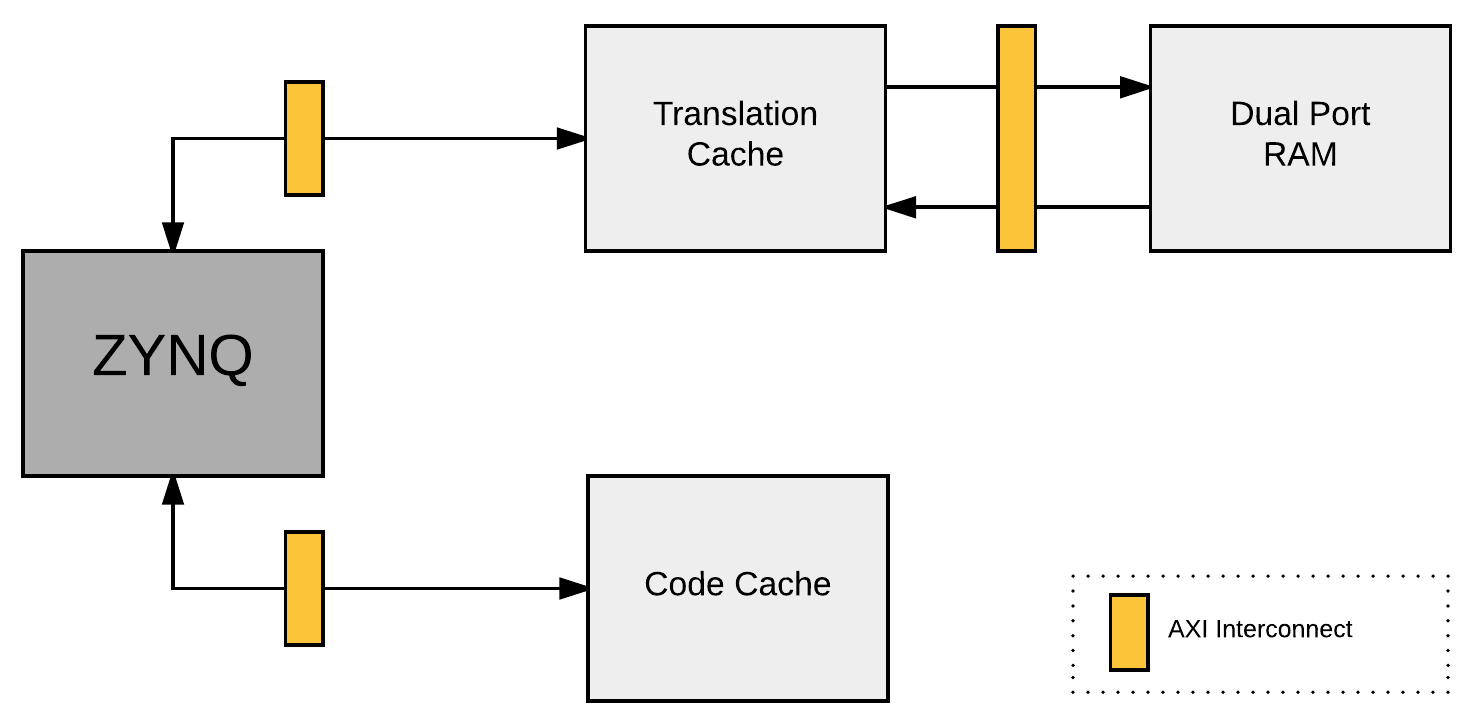
\includegraphics[scale = 0.2]{images/DesignHw1.png}
	\caption{Translation Cache hardware implementation with AXI Protocol}
	\label{fig:TCache_Hw}
\end{figure}

The first is represented in the figure \ref{fig:TCache_Hw} and probably less efficient is to create two AXI peripherals:
\begin{itemize}
	\item Translation Cache - Implemented AXI LITE peripheral;
	\item Dual Port RAM - Includes a BRAM Controller and a Block Memory Generator, both provided by Xilinx.	
\end{itemize}

For this implementation, the \textit{TCache} peripheral instantiate a CAM Module in order to find if the actual BB is or isn't translated and to return the address in the RAM where is the translation;